\documentclass[14pt,a4paper]{extarticle}

\usepackage{fontspec}
\usepackage[russian]{babel}
\setmainfont{Times New Roman}
\setsansfont{Arial}
\setmonofont{Times New Roman}[Scale=1]

\usepackage[left=30mm,right=15mm,top=20mm,bottom=20mm]{geometry}
\usepackage{setspace}
\usepackage{indentfirst}
\usepackage{amsmath}
\usepackage{booktabs}
\usepackage{hhline}
\usepackage{longtable}
\usepackage{array}
\usepackage{tabularx}
\usepackage{enumitem}
\usepackage{listings}
\usepackage{xcolor}
\usepackage{tikz}
\usepackage{pgfplots}
\pgfplotsset{compat=1.18}
\usepackage{float}
\usepackage{caption}
\usepackage{pdfpages}
\usepackage{pdflscape}
\usepackage{hyperref}
\usepackage{titlesec}
\urlstyle{same}

\addto\captionsrussian{\renewcommand{\contentsname}{СОДЕРЖАНИЕ}}

\usetikzlibrary{arrows.meta,positioning,shapes.geometric}

\onehalfspacing
\setlength{\parindent}{1.25cm}
\setlength{\parskip}{0pt}
\setlength{\emergencystretch}{3em}
\hyphenpenalty=10000
\exhyphenpenalty=10000
\sloppy
\clubpenalty=10000
\widowpenalty=10000
\displaywidowpenalty=10000
\setlength{\rightskip}{0.5mm}
\AtBeginDocument{%
    \setlength{\abovedisplayskip}{0pt}%
    \setlength{\abovedisplayshortskip}{0pt}%
    \setlength{\belowdisplayskip}{0pt}%
    \setlength{\belowdisplayshortskip}{0pt}%
}
\hypersetup{
    hidelinks,
    pdftitle={Сравнительный анализ ресурсной эффективности алгоритмов},
    pdfauthor={Ананьев Никита Андреевич}
}

\setlist[itemize]{
    label=---,
    labelindent=\parindent,
    leftmargin=*,
    nosep
}
\setlist[enumerate]{
    label=\arabic*),
    labelindent=\parindent,
    leftmargin=*,
    nosep
}

\titleformat{\section}[hang]
    {\normalfont\Large\bfseries\raggedright\hyphenpenalty=10000\exhyphenpenalty=10000}
    {\hspace*{1.25cm}\thesection}{\fontdimen2\font}{}
\titleformat{name=\section,numberless}[block]
    {\normalfont\Large\bfseries\centering\hyphenpenalty=10000\exhyphenpenalty=10000}
    {}{0pt}{}
\titleformat{\subsection}[hang]
    {\normalfont\large\bfseries\raggedright\hyphenpenalty=10000\exhyphenpenalty=10000}
    {\hspace*{1.25cm}\thesubsection}{\fontdimen2\font}{}
\titlespacing*{\section}{0pt}
    {0pt}{2.3ex plus .2ex}
\titlespacing*{\subsection}{0pt}
    {3.25ex plus 1ex minus .2ex}{1.5ex plus .2ex}

\newcommand{\structuralpart}[1]{%
    \clearpage
    \section*{#1}%
    \phantomsection
    \addcontentsline{toc}{section}{#1}%
}

\captionsetup{labelsep=endash}
\captionsetup[figure]{name=Рисунок,justification=centering}
\captionsetup[table]{name=Таблица,justification=raggedright,
    singlelinecheck=false,skip=2pt}
\setlength{\doublerulesep}{0.5pt}

\makeatletter
\renewcommand{\tagform@}[1]{%
    \maketag@@@{\kern1mm(\ignorespaces#1\unskip\@@italiccorr)\kern1mm}}
\renewcommand{\@biblabel}[1]{#1.}
\renewenvironment{thebibliography}[1]
    {\section*{\refname}%
     \@mkboth{\MakeUppercase\refname}{\MakeUppercase\refname}%
     \list{\@biblabel{\@arabic\c@enumiv}}%
          {\settowidth\labelwidth{\@biblabel{#1}}%
           \leftmargin\z@
           \itemindent\dimexpr\parindent+\labelwidth+\labelsep\relax
           \rightmargin 5mm
           \@openbib@code
           \usecounter{enumiv}%
           \let\p@enumiv\@empty
           \renewcommand\theenumiv{\@arabic\c@enumiv}}%
     \sloppy
     \clubpenalty4000
     \@clubpenalty\clubpenalty
     \widowpenalty4000
     \sfcode`\.\@m}
    {\def\@noitemerr
         {\@latex@warning{Empty `thebibliography' environment}}%
     \endlist}
\renewcommand*\l@section[2]{%
    \ifnum\c@tocdepth>\z@
        \addpenalty\@secpenalty
        \addvspace{.5em \@plus\p@}%
        \setlength\@tempdima{\dimexpr\parindent+1.5em\relax}%
        \begingroup
        \parindent\z@ \rightskip\@pnumwidth
        \parfillskip-\@pnumwidth
        \leavevmode\bfseries
        \advance\leftskip\@tempdima
        \hskip-\leftskip
        \hspace*{1.25cm}%
        #1\nobreak\hfil\nobreak
        \hb@xt@\@pnumwidth{\hss #2}\par
        \endgroup
    \fi}
\renewcommand*\l@subsection[2]{%
    \@dottedtocline{2}{1.25cm}{2.8em}{#1}{#2}}
\makeatother

\lstset{
    basicstyle=\normalfont\normalsize\rmfamily\setstretch{1},
    keywordstyle=\color{black},
    commentstyle=\color{black},
    stringstyle=\color{black},
    numbers=left,
    numberstyle=\normalfont\normalsize\rmfamily,
    stepnumber=1,
    numbersep=5pt,
    xleftmargin=9mm,
    linewidth=\dimexpr\linewidth-9mm\relax,
    frame=single,
    breaklines=true,
    columns=fullflexible,
    keepspaces=true,
    showstringspaces=false,
    tabsize=4
}
\renewcommand{\lstlistingname}{Листинг}

\tikzset{
    algorithm block/.style={draw,align=center,minimum width=64mm,
        inner xsep=0pt,inner ysep=2pt},
    terminator/.style={algorithm block,rectangle,rounded corners=5mm,
        minimum height=10mm},
    data/.style={trapezium,trapezium left angle=70,
        trapezium right angle=110,trapezium stretches=true,
        algorithm block,text width=54mm,minimum height=10mm},
    process/.style={algorithm block,rectangle,text width=54mm,
        minimum height=10mm},
    decision/.style={diamond,draw,align=center,aspect=3.2,
        minimum width=64mm,minimum height=20mm,inner sep=0pt},
    loop start/.style={rectangle,align=center,draw=none,
        minimum width=64mm,minimum height=12mm,text width=54mm,
        inner xsep=0pt,inner ysep=2pt,path picture={
            \draw[black]
                ([yshift=-5mm]path picture bounding box.north west) --
                ([xshift=5mm]path picture bounding box.north west) --
                ([xshift=-5mm]path picture bounding box.north east) --
                ([yshift=-5mm]path picture bounding box.north east) --
                (path picture bounding box.south east) --
                (path picture bounding box.south west) -- cycle;
        }},
    loop end/.style={rectangle,align=center,draw=none,
        minimum width=64mm,minimum height=12mm,text width=54mm,
        inner xsep=0pt,inner ysep=2pt,path picture={
            \draw[black]
                (path picture bounding box.north west) --
                (path picture bounding box.north east) --
                ([yshift=5mm]path picture bounding box.south east) --
                ([xshift=-5mm]path picture bounding box.south east) --
                ([xshift=5mm]path picture bounding box.south west) --
                ([yshift=5mm]path picture bounding box.south west) -- cycle;
        }},
    flow/.style={draw,-{Latex[length=2.5mm]}},
    every node/.style={font=\small}
}

\usepackage{graphicx}
\usetikzlibrary{shapes.misc,calc}
\hypersetup{pdftitle={Лабораторная работа № 4. Параллельная сегментация изображений},pdfauthor={Понарин А. А.}}
\tikzset{subroutine/.style={process,path picture={
\draw ([xshift=2mm]path picture bounding box.north west)--([xshift=2mm]path picture bounding box.south west);
\draw ([xshift=-2mm]path picture bounding box.north east)--([xshift=-2mm]path picture bounding box.south east);}},
every node/.style={font=\normalsize}}
\lstset{language=C,captionpos=b,breakatwhitespace=false,breakautoindent=false}
\makeatletter
\lst@AddToHook{Init}{\hyphenpenalty=0\relax\exhyphenpenalty=0\relax}
\makeatother
\setlength{\doublerulesep}{2pt}
\setcounter{tocdepth}{2}
\newcommand{\diagram}[3]{\begin{figure}[H]\centering\input{figures/#1.tex}\caption{#2}\label{#3}\end{figure}}
\begin{document}
\begin{titlepage}\thispagestyle{empty}
\noindent\begin{minipage}[c]{0.15\textwidth}
\includegraphics[width=\linewidth]{b_logo.jpg}\end{minipage}\hfill
\begin{minipage}[c]{0.83\textwidth}\centering\small
Министерство науки и высшего образования Российской Федерации\\
Федеральное государственное автономное образовательное учреждение\\высшего образования\\
«Московский государственный технический университет\\имени Н.~Э.~Баумана\\(национальный исследовательский университет)»\\
(МГТУ им. Н.~Э.~Баумана)
\end{minipage}
\par\vspace{4mm}\noindent\rule{\dimexpr\linewidth-1mm\relax}{1pt}\par\vspace{10mm}
\noindent ФАКУЛЬТЕТ «Информатика и системы управления»\\[4mm]
КАФЕДРА «Программная инженерия»
\vspace{23mm}
\begin{center}\Large\bfseries Лабораторная работа № 4\\[3mm]
по дисциплине «Анализ алгоритмов»\end{center}
\vspace{17mm}
\noindent Тема: «Последовательная и параллельная сегментация полутоновых изображений методом Оцу»
\par\vspace{15mm}
\noindent Студент: Понарин А.~А.\\[4mm]
Группа: ИУ7-55Б\\[4mm]
Преподаватели: Волкова Л.~Л., Строганов Д.~В.
\vfill\begin{center}2026~г.\end{center}
\end{titlepage}
\setcounter{page}{2}
\clearpage\tableofcontents
\structuralpart{ВВЕДЕНИЕ}
Полутоновое изображение представляет собой прямоугольную матрицу яркостей без цветовых каналов. Сегментацией называется разбиение его пикселей на классы. При пороговой сегментации классы определяются сравнением яркости с порогом. Такой способ применим к изображениям, для которых достаточно выделить две группы яркостей.

Цель работы --- разработать последовательный и параллельный алгоритмы сегментации полутоновых изображений, реализовать их и исследовать зависимость реального времени расчёта от числа рабочих потоков.

Для достижения цели необходимо:
\begin{itemize}
\item выбрать метод сегментации и определить входные и выходные данные;
\item разработать алгоритмы и схемы последовательного потока, диспетчера и рабочего потока;
\item реализовать алгоритмы на языке Си и выполнить функциональное тестирование;
\item измерить реальное время последовательной и параллельной реализаций при числе рабочих потоков от одного до восьмикратного числа логических ядер;
\item сравнить результаты и определить влияние размера изображения и числа рабочих потоков.
\end{itemize}

\clearpage\section{Аналитическая часть}
\subsection{Постановка задачи}
Дано полутоновое изображение шириной $W$ и высотой $H$, $W,H>0$. Пиксель --- элемент изображения; его яркость задаётся целым числом от 0 до 255. Число пикселей $N=W\cdot H$. Матрица хранится построчно в массиве $I=(I_0,\ldots,I_{N-1})$.

Требуется выбрать порог $T$ методом Оцу и получить бинарную маску $B$, то есть изображение с двумя значениями яркости:
\begin{equation}\label{eq:mask}
B_i=\begin{cases}0,&I_i\le T,\\255,&I_i>T,\end{cases}\qquad 0\le i<N.
\end{equation}
Нулём обозначается класс тёмных пикселей, значением 255 --- класс светлых. Связность областей и принадлежность конкретному анатомическому объекту не устанавливаются. Под чёрно-белым снимком понимается полутоновый исходник; уже бинарный вход также допустим.

\subsection{Метод Оцу}
Гистограмма яркостей $h[v]$ --- число пикселей со значением $v$. Метод Оцу основан на выборе порога, обеспечивающего наибольшее различие двух классов по яркости~\cite{otsu}. Для вычислений вводятся накопленные количества и суммы:
\begin{equation}\label{eq:sums}
\begin{aligned}
n_0(t)&=\sum_{v=0}^{t}h[v], & n_1(t)&=N-n_0(t),\\
s_0(t)&=\sum_{v=0}^{t}v\cdot h[v], & s&=\sum_{v=0}^{255}v\cdot h[v].
\end{aligned}
\end{equation}
Здесь $n_0,n_1$ --- размеры классов, $s_0$ --- сумма яркостей тёмного класса, $s$ --- сумма яркостей всего изображения. Средние яркости классов равны $\mu_0=s_0/n_0$ и $\mu_1=(s-s_0)/n_1$, если оба класса непусты. Межклассовая дисперсия определяется как
\begin{equation}
\sigma_B^2(t)=\frac{n_0(t)}{N}\cdot\frac{n_1(t)}{N}\cdot\bigl(\mu_0(t)-\mu_1(t)\bigr)^2.
\end{equation}
Для поиска максимума используется эквивалентный критерий без постоянного множителя $N^{-2}$:
\begin{equation}\label{eq:criterion}
J(t)=\frac{\bigl(N\cdot s_0(t)-n_0(t)\cdot s\bigr)^2}{n_0(t)\cdot n_1(t)},\qquad n_0(t)\cdot n_1(t)>0.
\end{equation}
Пороги перебираются от 0 до 254. Накопленные суммы обновляются за постоянное число действий на порог. При одинаковом значении критерия сохраняется меньший порог. Это принятое в работе правило разрешения равенства. Если изображение однотонное, непустое разбиение невозможно: порог принимается равным единственной яркости, маска получается нулевой.

\subsection{Возможности распараллеливания}
Построение гистограммы и применение готового порога требуют обхода всех пикселей. При непосредственном изменении общей гистограммы потребовалась бы синхронизация каждого приращения. Вместо этого каждый рабочий поток формирует собственные 256 счётчиков; после завершения этой фазы диспетчер суммирует их.

Порог зависит от всех локальных гистограмм. Поэтому бинаризацию нельзя начинать до окончания их объединения и поиска порога. После публикации порога каждый рабочий поток обрабатывает назначенный ему диапазон пикселей. Диапазоны разных потоков не перекрываются, поэтому два потока не записывают результат в один и тот же пиксель маски. Используется параллелизм по данным со статическим распределением пикселей.

Метод Оцу требует только гистограмму и не нуждается в заданном вручную пороге. Однако при неоднородном освещении и перекрывающихся распределениях яркости одной границы может быть недостаточно. В работе сравниваются реализации выбранной бинарной сегментации; точность выделения органов по клинической разметке не оценивается.

\clearpage\section{Конструкторская часть}
\subsection{Последовательный алгоритм}
В единственном потоке создаётся нулевая гистограмма, подсчитываются частоты яркостей, определяется порог по формуле~\eqref{eq:criterion} и формируется маска по формуле~\eqref{eq:mask}. На рисунке~\ref{fig:seq} приведена схема для допустимых входных данных; процедура выбора порога общая для обеих версий. Обозначение $[P]$ равно единице, если условие $P$ истинно, иначе нулю.
\diagram{sequential}{Схема алгоритма последовательного потока}{fig:seq}

\clearpage\subsection{Распределение работы}
Число рабочих потоков обозначается $q$. Диспетчер не входит в это число и не обрабатывает собственный участок изображения. Рабочему $j$, $0\le j<q$, назначается полуинтервал $[b_j,e_j)$:
\begin{equation}\label{eq:partition}
\begin{aligned}
d&=\lfloor N/q\rfloor,\quad r=N\bmod q,\\
b_j&=j\cdot d+\min(j,r),\\
e_j&=b_j+d+[j<r].
\end{aligned}
\end{equation}
Размеры участков различаются не более чем на один пиксель. Первый участок начинается с нуля, последний заканчивается на $N$, а конец каждого участка совпадает с началом следующего. Поэтому каждый пиксель обрабатывается ровно одним рабочим. При $q>N$ часть участков пуста, но фактически создаются все заданные $q$ потоков.

Для связи потоков используются мьютекс, то есть средство взаимоисключающего доступа к состоянию синхронизации, и две условные переменные для ожидания изменений этого состояния. Счётчик $c$ хранит число построенных гистограмм, флаг $p$ разрешает бинаризацию, флаг $a$ обозначает отмену запуска. Начальные значения равны нулю. Все обращения к этим переменным и публикация общего порога защищены одним мьютексом.

\subsection{Алгоритм потока-диспетчера}
После выделения памяти под локальные гистограммы и описатели создаются рабочие потоки. Диспетчер ожидает готовности всех гистограмм, объединяет их и вычисляет порог. Затем устанавливается флаг разрешения второй фазы, пробуждаются все ожидающие рабочие и освобождается мьютекс. Завершение каждого созданного потока ожидается до освобождения его данных. При неудачном запуске очередного рабочего устанавливается флаг отмены; уже созданные рабочие пробуждаются и завершаются без бинаризации.

На рисунке~\ref{fig:dispatcher} приведена схема диспетчера. Проверка аргументов и возврат при невозможности выделить или инициализировать служебные данные выполняются перед показанным запуском рабочих.
\diagram{dispatcher}{Схема алгоритма потока-диспетчера}{fig:dispatcher}

\clearpage\subsection{Алгоритм рабочего потока}
Используется один вид рабочего потока. Каждый рабочий получает свой участок изображения и маски, а также обнулённую диспетчером гистограмму. После подсчёта частот увеличивается $c$, уведомляется диспетчер и ожидается порог либо отмена. Затем независимо формируется участок маски. На рисунке~\ref{fig:worker} приведена схема рабочего потока.
\diagram{worker}{Схема алгоритма рабочего потока}{fig:worker}

\clearpage\subsection{Взаимодействие и корректность}
На рисунке~\ref{fig:interaction} представлен порядок взаимодействия потоков. Уведомления о готовности поступают после завершения соответствующей локальной гистограммы; второй этап разрешается только после получения всех уведомлений и вычисления общего порога.
\diagram{interaction}{Порядок взаимодействия диспетчера и рабочих потоков}{fig:interaction}

Ожидание условной переменной временно освобождает мьютекс; после пробуждения он вновь захватывается~\cite{posix}. Предикат ожидания проверяется в цикле, поэтому ложное пробуждение не разрешает преждевременную бинаризацию. После копирования порога мьютекс освобождается.

Локальные гистограммы принадлежат разным рабочим, поэтому при подсчёте частот конфликтов записи нет. Для каждого уровня яркости сумма локальных счётчиков совпадает со счётчиком последовательной версии. Суммирование целочисленное, порядок объединения результата не изменяет. В обеих версиях применяется одна процедура определения порога, включая правило выбора при равенстве критерия.

Видимость законченных гистограмм и вычисленного порога обеспечивается освобождением и захватом мьютекса. Для уведомлений о готовности и о продолжении используются разные условные переменные. Маска разбита на непересекающиеся участки; общий вход во время вычисления не изменяется. После ожидания завершения всех рабочих выходная маска полностью сформирована и побайтно совпадает с последовательным результатом.

\subsection{Оценка затрат ресурсов}
Пусть $L=256$ --- число уровней яркости. Последовательная трудоёмкость составляет $O(N+L)$, дополнительная память без учёта входа и маски --- $O(L)$. Суммарная работа параллельной версии равна $O(N+q\cdot L)$, дополнительная память --- $O(q\cdot L+q)$. Для маски в обеих версиях требуется ещё $N$ байт.

При одновременном исполнении всех рабочих и равномерной загрузке оценка вычислительной части критического пути равна
\begin{equation}
O\bigl(\lceil N/q\rceil+q\cdot L+L\bigr).
\end{equation}
К реальному времени добавляются расходы на выделение памяти, запуск, синхронизацию и завершение потоков. При $q$ больше числа доступных логических ядер все рабочие одновременно не исполняются, поэтому член $N/q$ не описывает фактическое сокращение времени. Объединение гистограмм и поиск порога остаются последовательными этапами.

\subsection{Требования к программе и тестирование}
Программа читает и записывает двоичные полутоновые изображения PGM с сигнатурой P5 и максимальным значением 255. Нулевые размеры, переполнение размера, усечённый растр, лишние байты и неподдерживаемый формат отклоняются. Число рабочих потоков задаётся явно в диапазоне от 1 до 4096. В библиотечных функциях допускается использование одного буфера для входа и результата; частичное перекрытие буферов не допускается.

Для проверки выбраны изображения с заранее определяемыми порогом и маской: однотонные, бинарные, с двумя различными яркостями и со всеми уровнями серого. В обоих режимах сравнивались порог и значения пикселей полученной маски. Примеры проверок приведены в таблице~\ref{tab:tests}; векторы рассматриваются как изображения высотой один пиксель.
\begin{table}[H]\caption{Примеры функциональных проверок}\label{tab:tests}
\centering\begin{tabularx}{\textwidth}{|X|c|X|}\hline
Вход & Порог & Маска / результат\\\hhline{|=:=:=|}
$(0)$ & 0 & $(0)$\\\hline
$(255)$ & 255 & $(0)$\\\hline
15 пикселей яркости 77 & 77 & все значения 0\\\hline
$(0,255)$ & 0 & $(0,255)$\\\hline
$(10,10,200,200)$ & 10 & $(0,0,255,255)$\\\hline
$(0,2,4)$ & 0 & $(0,255,255)$\\\hline
$(0,1,\ldots,255)$ & 127 & 128 нулей, 128 значений 255\\\hline
Нулевой размер, усечённый PGM & --- & ошибка ввода\\\hline
$q=0$, $q=-1$, $q=4097$ & --- & ошибка аргумента\\\hline
\end{tabularx}\end{table}

На однотонном изображении проверялось получение нулевой маски, на бинарном --- сохранение разделения на чёрные и белые пиксели. Для входа $(0,2,4)$ проверялся выбор меньшего порога при равенстве критерия.

Последовательная и параллельная версии дали одинаковые результаты. Дополнительно проверялись случаи, когда размер изображения не делится на число потоков и когда потоков больше, чем пикселей. При неверном числе потоков, нулевом размере и усечённом изображении программа выдавала сообщение об ошибке.

\clearpage\section{Технологическая часть}
\subsection{Средства реализации}
Реализации написаны на языке Си (C), стандарт 2011 года (C11). Для потоков, мьютекса и условных переменных применяется интерфейс потоков POSIX в реализации winpthreads, поставляемой с MSYS2. Использован компилятор GCC 14.2.0, среда UCRT64. Измерительная сборка выполняется с параметрами \texttt{-std=c11 -O0 -Wall -Wextra -Wpedantic -pthread}, без отладочной информации и без оптимизации.

Счётчики гистограммы имеют тип беззнакового 64-разрядного целого числа. Размер изображения ограничен условием $N\le\lfloor(2^{64}-1)/255\rfloor$ и доступной памятью. Это исключает переполнение суммы яркостей. Критерий Оцу вычисляется с использованием вещественного типа расширенной точности \texttt{long double}; поэтому для практически равных максимумов на иных больших входах округление может влиять на выбранный порог. В функциональных проверках совпадение с точным эталоном подтверждено. Между последовательной и параллельной версиями порядок вычисления критерия одинаков.

Исходные тексты разделены на модули сегментации, обработки изображений и командного интерфейса. Основные функции подключены непосредственно из исходных файлов в приложении~А. Один локальный массив гистограммы занимает 2048 байт, $q$ таких массивов --- $2048\cdot q$ байт. Дополнительно выделяются описатели потоков и структуры синхронизации; память стеков управляется библиотекой потоков и операционной системой.

\subsection{Пример сегментации}
На рисунке~\ref{fig:example} представлены сгенерированный полутоновый фантом и его бинарная маска. Фантом составлен из эллиптических областей двух диапазонов яркости с псевдослучайным шумом; он служит воспроизводимым учебным входом и не является рентгеновским снимком пациента. Для размера $512\times512$ получен порог $T=64$. Последовательная и параллельная маски совпали.
\begin{figure}[H]\centering
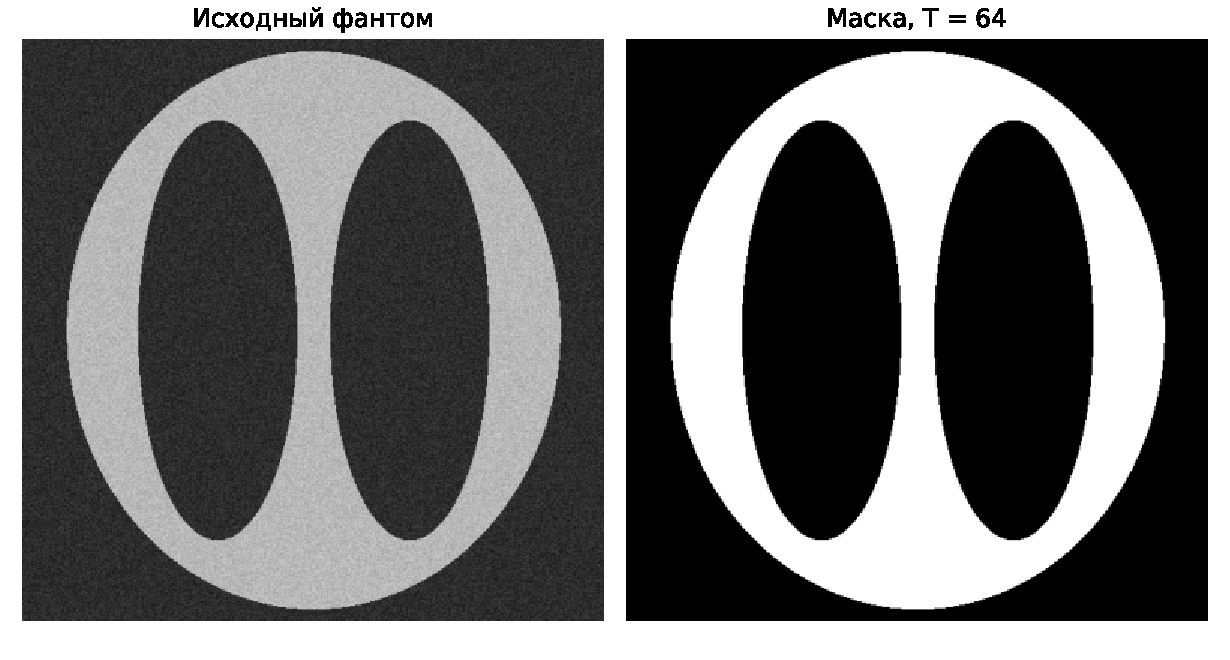
\includegraphics[width=\textwidth]{figures/example.pdf}
\caption{Исходный синтетический фантом и результат сегментации}\label{fig:example}
\end{figure}

\clearpage\section{Исследовательская часть}
\subsection{Условия проведения исследования}
Замеры проводились на следующей конфигурации:
\begin{itemize}
\item процессор: Intel Core i3-1115G4, 3,00 ГГц, два физических и четыре логических ядра;
\item оперативная память: 7,75 ГиБ;
\item операционная система: Windows 11;
\item компилятор: GCC 14.2.0 с флагом \texttt{-O0}.
\end{itemize}

\subsection{Методика замеров}
Для каждого сочетания размера изображения и числа потоков выполнялось 100 повторений, после чего вычислялось среднее арифметическое. Реальное время полного расчёта измерялось с помощью QueryPerformanceCounter~\cite{timer}. Создание, синхронизация и завершение рабочих потоков учитывались; генерация изображения и файловый ввод-вывод в замер не включались.

Использовались квадратные полутоновые изображения со сторонами 256, 512, 1024, 2048 и 4096 пикселей. Для каждого размера обеим версиям передавалось одно и то же изображение. Число рабочих потоков $q\in\{1,2,4,8,16,32\}$ соответствует диапазону от одного до $8\cdot k$, где $k=4$ --- число логических ядер. Помимо параллельной версии при одном рабочем потоке отдельно измерялась последовательная версия.

\subsection{Результаты замеров}
В таблице~\ref{tab:sizes} представлены средние времена последовательной версии и параллельной версии при одном рабочем потоке.
\begin{table}[H]\caption{Сравнение реализаций при разных размерах}\label{tab:sizes}
\centering\begin{tabularx}{\textwidth}{|c|X|X|}\hline
Сторона, пиксель & Послед., мс & Паралл., $q=1$, мс\\\hhline{|=:=:=|}
256 & 0,186 & 0,401 \\\hline
512 & 0,701 & 1,075 \\\hline
1024 & 3,538 & 4,900 \\\hline
2048 & 34,857 & 46,870 \\\hline
4096 & 132,034 & 173,095 \\\hline
\end{tabularx}\end{table}

На рисунке~\ref{fig:time} представлена зависимость времени от размера изображения для всех исследованных конфигураций. Обе оси имеют логарифмический масштаб.
\begin{figure}[H]\centering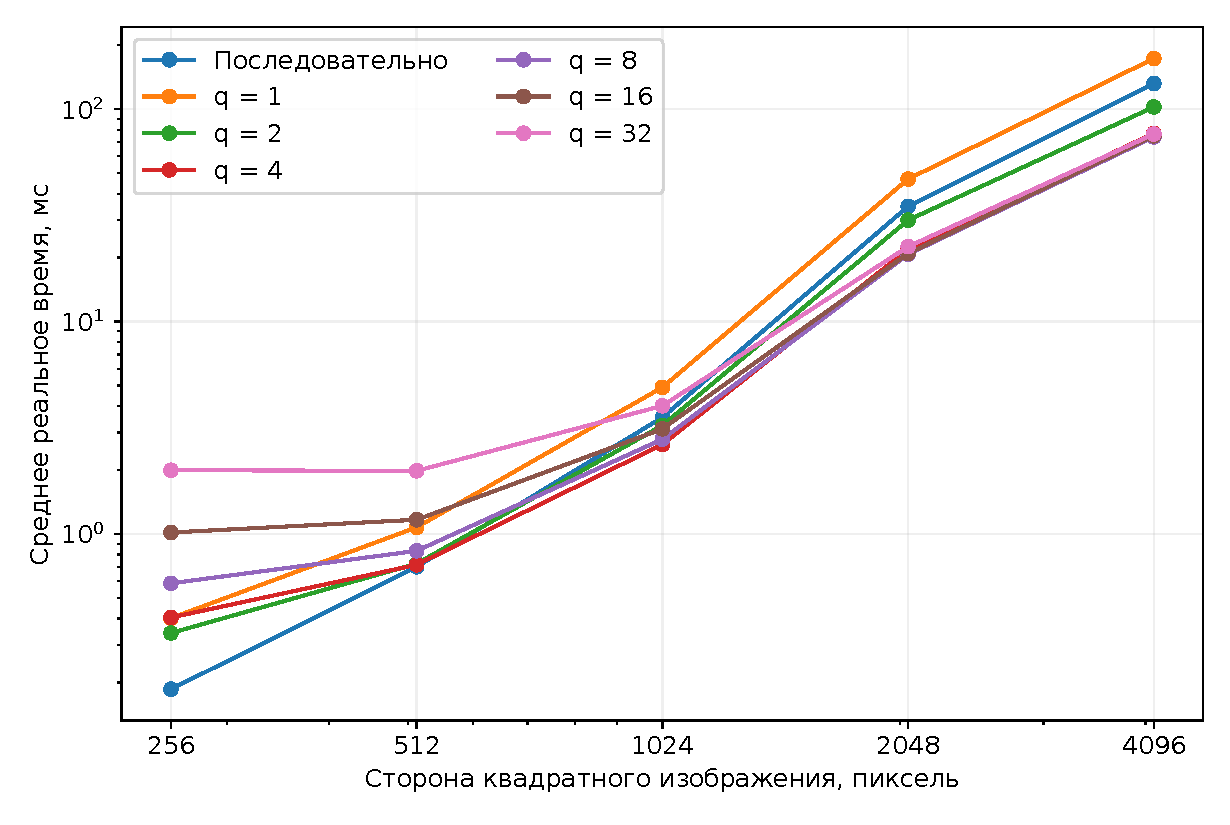
\includegraphics[width=\textwidth]{figures/time.pdf}
\caption{Зависимость среднего реального времени от размера изображения}\label{fig:time}\end{figure}

Для изображения $4096\times4096$ результаты при разном числе рабочих потоков приведены в таблице~\ref{tab:q}. Ускорение рассчитывается как отношение среднего времени последовательной версии к среднему времени параллельной версии. Полные результаты приведены в приложении~Б.
\begin{table}[H]\caption{Результаты для изображения $4096\times4096$}\label{tab:q}
\centering\begin{tabularx}{\textwidth}{|c|X|X|}\hline
Рабочие потоки & Время, мс & Ускорение\\\hhline{|=:=:=|}
1 & 173,095 & 0,76 \\\hline
2 & 102,399 & 1,29 \\\hline
4 & 76,934 & 1,72 \\\hline
8 & 73,955 & 1,79 \\\hline
16 & 74,901 & 1,76 \\\hline
32 & 76,335 & 1,73 \\\hline
\end{tabularx}\end{table}

На рисунке~\ref{fig:speedup} представлена зависимость ускорения от числа рабочих потоков. Значения меньше единицы соответствуют замедлению.
\begin{figure}[H]\centering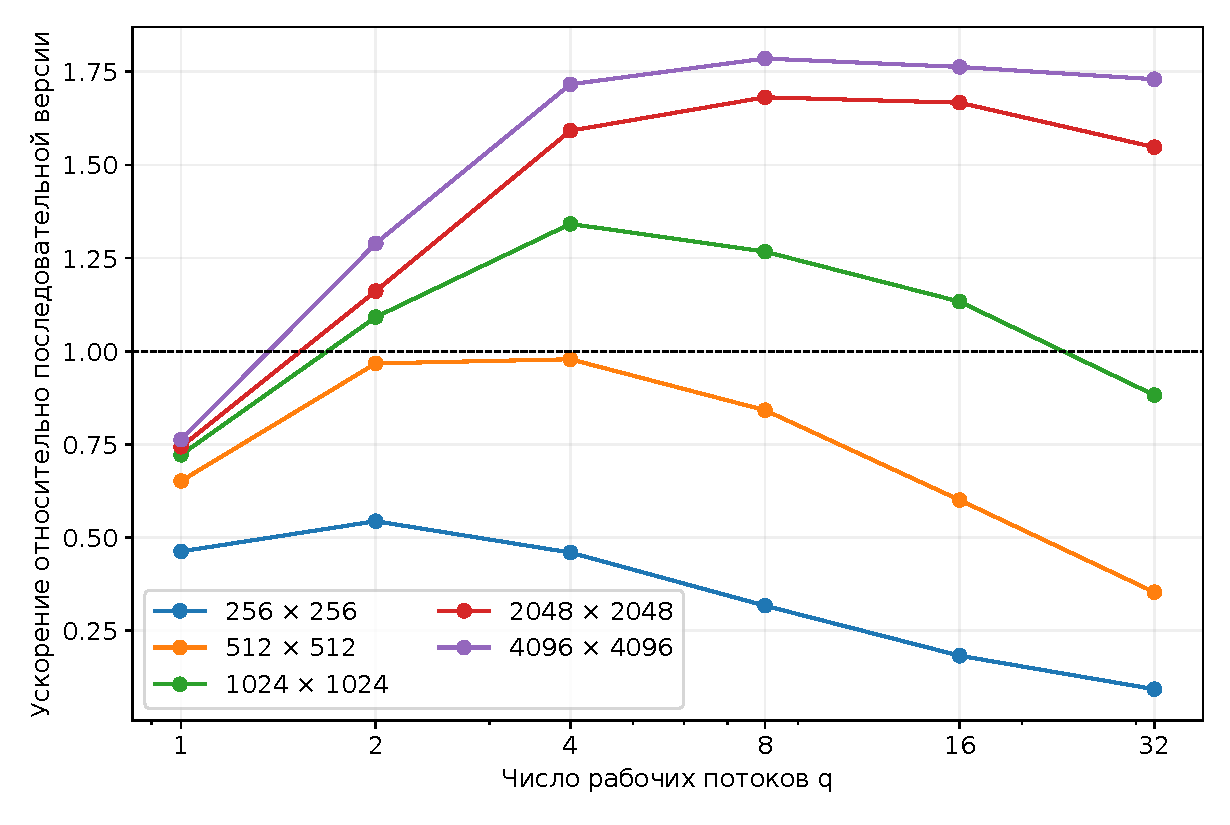
\includegraphics[width=\textwidth]{figures/speedup.pdf}
\caption{Ускорение параллельной реализации при разных размерах}\label{fig:speedup}\end{figure}

\subsection{Анализ результатов}
На изображениях $256\times256$ и $512\times512$ параллельная версия не дала выигрыша: расходы на управление потоками превышают сокращение времени обработки пикселей. Начиная с $1024\times1024$ в исследованном наборе получено ускорение при нескольких рабочих потоках.

При одном рабочем потоке параллельная версия медленнее последовательной для всех размеров. Для $4096\times4096$ время увеличилось с 132,034 до 173,095 мс, то есть примерно на 31\,\%.

Для наибольшего изображения минимальное среднее время получено при восьми рабочих потоках: 73,955 мс, ускорение 1,79. Дальнейшее увеличение числа потоков заметного выигрыша не дало. Результаты при 4, 8, 16 и 32 потоках близки с учётом разброса измерений, поэтому устойчивое преимущество восьми потоков не утверждается. Замеры выполнялись в обычной настольной среде без фиксации частоты процессора.

\structuralpart{ЗАКЛЮЧЕНИЕ}
В ходе работы получены следующие результаты:
\begin{itemize}
\item выбран метод Оцу, определены полутоновое исходное изображение и бинарная маска результата, зафиксированы правила обработки однотонного входа и одинаковых максимумов критерия;
\item разработаны последовательный и параллельный алгоритмы, схемы единственного последовательного потока, диспетчера и одного вида рабочих потоков с двумя зависимыми фазами;
\item выполнены реализации на языке Си11, проверены типовые и граничные случаи, совпадение результатов обеих версий и обработка неверного ввода;
\item выполнены замеры реального времени для пяти размеров изображений, самостоятельной последовательной версии и параллельной версии при 1, 2, 4, 8, 16 и 32 рабочих потоках;
\item установлено, что для небольших входов параллельная версия замедляет расчёт, а для $4096\times4096$ минимальное наблюдавшееся среднее время получено при восьми рабочих с ускорением 1,79; дальнейшее увеличение числа потоков устойчивого выигрыша не дало.
\end{itemize}

\clearpage
\renewcommand{\refname}{СПИСОК ИСПОЛЬЗОВАННЫХ ИСТОЧНИКОВ}
\phantomsection\addcontentsline{toc}{section}{СПИСОК ИСПОЛЬЗОВАННЫХ ИСТОЧНИКОВ}
\begin{thebibliography}{3}
\bibitem{otsu} Оцу Н. Метод выбора порога по гистограммам уровней серого (A Threshold Selection Method from Gray-Level Histograms) // Труды Института инженеров электротехники и электроники по системам, человеку и кибернетике (IEEE Transactions on Systems, Man, and Cybernetics). 1979. Т. SMC-9, № 1. С. 62--66. DOI: \href{https://doi.org/10.1109/TSMC.1979.4310076}{10.1109/TSMC.1979.4310076}.
\bibitem{posix} Открытая группа (The Open Group). Ожидание условной переменной (pthread\_cond\_wait) // Базовые спецификации, выпуск 8, 2024. URL: \url{https://pubs.opengroup.org/onlinepubs/9799919799/functions/pthread_cond_wait.html} (дата обращения: 12.11.2026).
\bibitem{timer} Майкрософт (Microsoft). Функция счётчика высокой точности (QueryPerformanceCounter). URL: \url{https://learn.microsoft.com/en-us/windows/win32/api/profileapi/nf-profileapi-queryperformancecounter} (дата обращения: 12.11.2026).
\end{thebibliography}
\structuralpart{ПРИЛОЖЕНИЕ А}
\begin{center}Основные исходные тексты\end{center}
\renewcommand{\thelstlisting}{А.\arabic{lstlisting}}
\setcounter{lstlisting}{0}
В листинге~\ref{lst:api} «Интерфейс функций сегментации» приведены объявления типов и функций. В листинге~\ref{lst:implementation} «Реализация метода Оцу и управления потоками» приведён исходный код вычислительного модуля, использованного при тестировании и измерениях.
\lstinputlisting[caption={Интерфейс функций сегментации},label={lst:api}]{src/segmentation.h}
\clearpage
\lstinputlisting[caption={Реализация метода Оцу и управления потоками},label={lst:implementation}]{src/segmentation.c}

\structuralpart{ПРИЛОЖЕНИЕ Б}
\begin{center}Полные результаты измерений\end{center}
\renewcommand{\thetable}{Б.\arabic{table}}\setcounter{table}{0}
В таблице~\ref{tab:all} представлены сводные результаты всех конфигураций. В столбце $q$ обозначением «Послед.» отмечена самостоятельная последовательная реализация. Для каждой строки учтено 100 измерений, время приведено в миллисекундах. Минимум и максимум характеризуют отдельные вызовы, а не доверительный интервал среднего.
\begin{longtable}{|p{23mm}|p{29mm}|p{26mm}|p{26mm}|p{26mm}|}
\caption{Полные результаты измерений}\label{tab:all}\\\hline
$q$ & Среднее & Станд. откл. & Минимум & Максимум\\\hhline{|=:=:=:=:=|}
\endfirsthead
\multicolumn{5}{l}{Продолжение таблицы~\thetable}\\\hline
$q$ & Среднее & Станд. откл. & Минимум & Максимум\\\hhline{|=:=:=:=:=|}
\endhead
\multicolumn{5}{|c|}{Изображение $256 \times 256$}\\\hline
Послед. & 0,186 & 0,020 & 0,174 & 0,251 \\\hline
1 & 0,401 & 0,085 & 0,327 & 0,826 \\\hline
2 & 0,342 & 0,071 & 0,267 & 0,628 \\\hline
4 & 0,404 & 0,095 & 0,322 & 0,887 \\\hline
8 & 0,586 & 0,081 & 0,484 & 0,897 \\\hline
16 & 1,015 & 0,217 & 0,816 & 2,488 \\\hline
32 & 1,995 & 0,570 & 1,586 & 5,907 \\\hline
\multicolumn{5}{|c|}{Изображение $512 \times 512$}\\\hline
Послед. & 0,701 & 0,046 & 0,670 & 0,869 \\\hline
1 & 1,075 & 0,122 & 1,000 & 2,158 \\\hline
2 & 0,724 & 0,167 & 0,593 & 1,702 \\\hline
4 & 0,716 & 0,187 & 0,620 & 2,181 \\\hline
8 & 0,832 & 0,115 & 0,742 & 1,486 \\\hline
16 & 1,166 & 0,187 & 1,018 & 1,990 \\\hline
32 & 1,982 & 0,296 & 1,730 & 2,963 \\\hline
\multicolumn{5}{|c|}{Изображение $1024 \times 1024$}\\\hline
Послед. & 3,538 & 1,904 & 2,654 & 9,319 \\\hline
1 & 4,900 & 2,750 & 3,615 & 13,763 \\\hline
2 & 3,242 & 1,841 & 1,897 & 9,761 \\\hline
4 & 2,638 & 1,473 & 1,874 & 9,245 \\\hline
8 & 2,793 & 1,544 & 1,983 & 8,101 \\\hline
16 & 3,123 & 1,766 & 2,242 & 13,246 \\\hline
32 & 4,011 & 2,020 & 2,786 & 11,782 \\\hline
\multicolumn{5}{|c|}{Изображение $2048 \times 2048$}\\\hline
Послед. & 34,857 & 6,053 & 16,462 & 45,279 \\\hline
1 & 46,870 & 8,813 & 22,562 & 81,897 \\\hline
2 & 30,017 & 7,893 & 12,983 & 60,721 \\\hline
4 & 21,900 & 4,963 & 10,222 & 47,354 \\\hline
8 & 20,732 & 4,466 & 9,916 & 44,206 \\\hline
16 & 20,913 & 4,471 & 9,918 & 44,469 \\\hline
32 & 22,526 & 7,737 & 11,221 & 85,670 \\\hline
\multicolumn{5}{|c|}{Изображение $4096 \times 4096$}\\\hline
Послед. & 132,034 & 21,368 & 70,160 & 182,776 \\\hline
1 & 173,095 & 25,124 & 100,864 & 259,892 \\\hline
2 & 102,399 & 19,625 & 60,640 & 150,750 \\\hline
4 & 76,934 & 12,599 & 48,247 & 130,949 \\\hline
8 & 73,955 & 10,001 & 49,148 & 91,837 \\\hline
16 & 74,901 & 8,838 & 45,157 & 90,180 \\\hline
32 & 76,335 & 8,286 & 57,570 & 103,123 \\\hline
\end{longtable}

\end{document}
